\documentclass[aspectratio=169]{beamer}
\usepackage{polski}
\usepackage[utf8]{inputenc} % utf8
\usepackage{xspace}
\usepackage[autostyle]{csquotes} 
\usepackage{textpos}
\newcommand{\wiki}[1]{https://pl.wikipedia.org/wiki/Teksel}

\newcommand{\DICOM}[0]{\mbox{DICOM}\xspace}

\def\zerospace{\hspace{0px}}
\def\scopedots{\zerospace::\zerospace}

\def\sokarprefix{Sokar\scopedots}
\newcommand{\sokarclass}[1]{\textit{\sokarprefix#1}}
\newcommand{\sokarfunction}[2]{\textit{\sokarprefix#1\scopedots#2()}}

\def\gdcmprefix{gdcm\scopedots}
\def\gdcmdocurl{http://gdcm.sourceforge.net/html}
\newcommand{\gdcmclass}[1]{\textit{\href{\gdcmdocurl/classgdcm_1_1#1.html}{\gdcmprefix#1}}}
\newcommand{\gdcmfunction}[2]{\textit{\href{\gdcmdocurl/classgdcm_1_1#1.html\##2}{\gdcmprefix#1\scopedots#2()}}}

\def\qtprefix{Qt\scopedots}
\def\qtdocurl{https://doc.qt.io/qt-5}
\newcommand{\qtclass}[1]{\textit{\lowercase{\href{\qtdocurl/#1.html}}{\qtprefix#1}}}
\newcommand{\qtfunction}[2]{\textit{\lowercase{\href{\qtdocurl/#1.html\##2}}{\qtprefix#1\scopedots#2()}}}

\def\stdprefix{std\scopedots}
\newcommand{\stdclass}[2]{\href{https://en.cppreference.com/w/cpp/#2}{\stdprefix#1}}

\newcommand{\dicomvr}[1]{VR:#1}

\def\dicomtagprefix{{\small$^\text{Dicom}_\text{Tag}$}\xspace}
\def\dicomtagurl#1{\url{https://duckduckgo.com/?q=!ducky+#1+site\3Adicom.innolitics.com}}
\newcommand{\dicomtag}[3]{\href{https://duckduckgo.com/?q=!ducky+DICOM+Tag+#1+(#2,#3)+site\%3Adicom.innolitics.com}{\dicomtagprefix#1 (0x#2, 0x#3)}}

\newenvironment{conditions}
{\par\vspace{\abovedisplayskip}\noindent\begin{tabular}{>{$}l<{$} @{${}={}$} l}}
        {\end{tabular}\par\vspace{\belowdisplayskip}}

\def\quotett#1{\enquote{\texttt{#1}}}
\def\cppcode#1{{\color{blue}\texttt{#1}}}
\def\keyword#1{{\textbf{#1}}}
\def\dataword#1{{\color{gray}\enquote{\texttt{#1}}}}

% \renewcommand\paragraph{%
%     \@startsection{paragraph}{4}{0mm}%
%        {-\baselineskip}%
%        {.5\baselineskip}%
%        {\normalfont\normalsize\bfseries}}


\newcommand{\fromEng}[1]{(ang. \textit{#1})}


\newenvironment{infobox}[1][]
{\begin{mdframed}[
            frametitle={#1},
            skipabove=\baselineskip plus 2pt minus 1pt,
            skipbelow=\baselineskip plus 2pt minus 1pt,
            frametitleaboveskip= 7pt,
            frametitlebelowskip= 7pt,
            linewidth=1pt,
            linecolor=black,
            frametitlerule=false,
            frametitlebackgroundcolor=blue!10,
            backgroundcolor=blue!10,
            roundcorner=7pt,
            nobreak=true
        ]}
        {\end{mdframed}}

\newenvironment{zeroindent}
{\par\setlength{\parindent}{0pt}}
{\par}


\def\qtclassExplanations{
    \begin{infobox}
        \begin{zeroindent}
            W dokumencie są wielokrotnie zawarte odniesienia do klas z biblioteki Qt.
            Dlatego, aby zwiększyć czytelność pracy, została zastosowana konwencja poprzedzania klas z biblioteki Qt przedrostkiem \textit{\qtprefix}, który jest za razem przestrzenią nazw.
            Przykład poniżej:

            \begin{center}
                \qtclass{QObject}
            \end{center}

            Wszystkie funkcje wewnątrz klas są oznaczone następująco:

            \begin{center}
                \qtfunction{QObject}{connect}
            \end{center}

            Dodatkowo w dokumencie PDF klikając na nazwę klasy użytkownik zostanie przekierowany do oficjalnej dokumentacji Qt znajdującej się pod adresem \url{\qtdocurl}.
        \end{zeroindent}
    \end{infobox}
}

\def\gdcmclassExplanations{
    \begin{infobox}
        \begin{zeroindent}
            W dokumencie są wielokrotnie zawarte odniesienia do klas z biblioteki GDCM.
            Dlatego, aby zwiększyć czytelność pracy, została zastosowana konwencja poprzedzania klas z biblioteki Qt przedrostkiem \textit{\gdcmprefix}, który za razem jest przestrzenią nazw biblioteki.
            Przykład poniżej:

            \begin{center}
                \gdcmclass{ImageReader}
            \end{center}

            Wszystkie funkcje wewnątrz klas są oznaczone następująco:

            \begin{center}
                \gdcmfunction{ImageReader}{GetImage}
            \end{center}

            Dodatkowo w dokumencie PDF można kliknąć na nazwę klasy i użytkownik zostanie przekierowany do oficjalnej dokumentacji GDCM znajdującej się pod adresem \url{\gdcmdocurl}.
        \end{zeroindent}
    \end{infobox}
}

\def\sokarclassExplanations{
    \begin{infobox}
        \begin{zeroindent}
            W dokumencie są wielokrotnie zawarte odniesienia do klas z przeglądarki obrazów.
            Dlatego, aby zwiększyć czytelność pracy, została zastosowana konwencja poprzedzania klas z aplikacji przedrostkiem \textit{\sokarprefix}, który za razem jest przestrzenią nazw programu.
            Przykład poniżej:

            \begin{center}
                \sokarclass{DataConverter}
            \end{center}

            Wszystkie funkcje wewnątrz klas są oznaczone następująco:

            \begin{center}
                \sokarfunction{DataConverter}{toString}
            \end{center}

            Dodatkowo w dokumencie PDF można kliknąć na nazwę klasy i użytkownik zostanie przekierowany do TU WYMYŚLIĆ DO CZEGO
        \end{zeroindent}
    \end{infobox}
}

\def\dicomtagExplanations{
    \begin{infobox}
        \begin{zeroindent}
            W dokumencie są wielokrotnie zawarte odniesienia do znaczników \DICOM.
            Dlatego aby zwiększyć czytelność pracy, została zastosowana konwencja poprzedzania znaczników przedrostkiem \dicomtagprefix i sufiksem składającym się z numeru grupy i elementu grupy zapisanych heksadecymalnie.
            Przykład poniżej:

            \begin{center}
                \dicomtag{PatientID}{0010}{0020}
            \end{center}

            Oznacza to, że jest to znacznik o słowie kluczowym \enquote{PatientID}, numerze grupy $10_{16}$ i numerze elementu $20_{16}$. 

            Wyrażenie \enquote{informacja ta zawarta w znaczniku \dots} będzie oznaczało, że ta informacja znajduje się w elemencie danych o znaczniku.

            Dodatkowo w dokumencie PDF można kliknąć na nazwę klasy i użytkownik zostanie przekierowany do strony \url{https://dicom.innolitics.com/ciods} poprzez wyszukiwarkę DuckDuckGo, na której znajduje się przeglądarka znaczników \DICOM.
        \end{zeroindent}
    \end{infobox}
}

\def\dicomRetired{
    \begin{infobox}
        \begin{zeroindent}
            Wiele elementów danych lub wartości zostały wycofane ze standardu \DICOM w wersji 3.0.
            Oznaczane są jako wycofane \fromEng{retired}.
            Można dalej wspierać ich obsługę w celach wstecznej kompatybilności, ale nie jest to wymagane.
        \end{zeroindent}
    \end{infobox}
}


%%%%%%%%%%%%%%%%%%%%%%%%%%%%%%%%%%%%%%%%%%%%%%%%%%%%%%%%%%%%%%%%%%%%%%%%%%%%%%%%
% Pakiet do kolorowania składni

\usepackage{listings}

%https://www.overleaf.com/learn/latex/Code_listing
\lstdefinestyle{cppstyle}{
    language=C++,
    backgroundcolor=\color{white},   
    commentstyle=\color{teal},
    keywordstyle=\color{blue},
    numberstyle=\tiny\color{black},
    stringstyle=\color{red},
    basicstyle=\ttfamily\scriptsize,
    breakatwhitespace=false,
    breaklines=true,
    captionpos=b,
    keepspaces=true,
    numbers=left,
    numbersep=5pt,
    showspaces=false,
    showstringspaces=false,
    showtabs=false,
    tabsize=4,
    inputencoding=utf8,
    extendedchars=true,
    morekeywords={
        override,
        qreal, emit, slots, signals,
        qint8, qint16, qint32, qint64,
        quint8, quint16, quint32, quint64,
    },
    literate={ą}{{\k{a}}}1 {ć}{{\'{c}}}1 {ę}{{\k{e}}}1 {Ł}{{\L{}}}1 {ł}{{\l{}}}1 {ń}{{\'{n}}}1 {ó}{{\'{o}}}1 {ś}{{\'{s}}}1 {ż}{{\.{z}}}1 {ź}{{\'{z}}}1 ,
}

\lstset{style=cppstyle}


\newcommand*{\thead}[1]{\multicolumn{1}{|c|}{\bfseries #1}}
\def\dicomtagprefix{}

\usetheme{Boadilla}
\definecolor{WEITI_grafitowy}{rgb}{0.235294118, 0.235294118, 0.298039216}
\usecolortheme[named=WEITI_grafitowy]{structure}

\title{Wieloplatformowa przeglądarka obrazów DICOM w C++}
\author{Adam Jędrzejowski}
\date{\today}
\institute[]{
    Wydział Elektroniki i Technik Informacyjnych Politechniki Warszawskiej\\
    Instytut Radioelektroniki i Technik Multimedialnych\\ 
    Zakład Elektroniki Jądrowej i Medycznej}

\begin{document}

\begin{frame}

    \begin{textblock*}{0mm}(0.5cm,0cm)
        
\includegraphics[height=0.8cm]{img/logo-weiti.png}
    \end{textblock*}
    \vspace{1cm}
    \titlepage
\end{frame}

% logo wydziału
\addtobeamertemplate{frametitle}{}{%
    \begin{textblock*}{0mm}(11.2cm,-0.5cm)
        
\includegraphics[height=0.8cm]{img/logo-weiti.png}
    \end{textblock*}}

\addtobeamertemplate{frametitle}{\vspace*{0cm}}{\vspace*{0.3cm}}


\begin{frame}
    \frametitle{Obrazowe techniki medyczne}

    \begin{itemize}
        \item Radiografia --- RTG
        \item Tomografia komputerowa --- CT
        \item Obrazowanie metodą rezonansu magnetycznego --- MRI
        \item Ultrasonografia
        \item Scyntygrafia
        \item Tomografia SPECT
        \item Tomografia PET
    \end{itemize}
\end{frame}

\begin{frame}[t]
    \frametitle{Standard DICOM}
    \begin{columns}[t]
        \column{0.4\textwidth}

        \scriptsize
        \vspace{-7em}
        Standard DICOM jest odpowiedzią społeczności radiologów, radiofarmaceutów, fizyków medycznych na potrzebę wymiany danych pomiędzy różnymi systemami komputerowymi, przeglądarek obrazów, stacji do przetwarzania i analizowania obrazów medycznych.

        \vspace{1em}
        Standard \DICOM v3 definiuje ujednolicony sposób zapisu i przekazywania danych medycznych reprezentujących lub związanych z obrazami diagnostycznymi w medycynie.

        \vspace{1em}
        W obecnej chwili standard DICOM definiuje 81 różnych typów badań.

        \vspace{1em}
        Plik w formacie \DICOM przypomina zbiór elementów danych z rekordami.
        Zbiór nazywa się \enquote{Data Set} i składa się z rekordów, które nazywają się \enquote{Data Element}.
        Elementy danych są ułożone w postaci listy.
        Element danych może zawierać w sobie listę elementów danych.

        \column{0.6\textwidth}
        \tiny
        \begin{tabular}{|l|c|c|l|}
            \hline
            \thead{Nazwa}             & \thead{Identyfikator} & \thead{Typ danych} & \thead{Opis}                \\\hline
            SpecificCharacterSet      & (0008,0005)           & CS                 & Używana specyfikacja        \\\hline
            InstitutionName           & (0008,0080)           & LO                 & Miejsce wykonywania badania \\\hline
            Manufacturer              & (0008,0070)           & LO                 & Producent aplikacji         \\\hline
            StationName               & (0008,1010)           & SH                 & Nazwa urządzenia            \\\hline
            PatientID                 & (0010,0020)           & LO                 & Identyfikator pacjenta      \\\hline
            PatientsName              & (0010,0010)           & PN                 & Nazwisko pacjenta           \\\hline
            PatientsBirthDate         & (0010,0030)           & DA                 & Data urodzin pacjenta       \\\hline
            PatientsSex               & (0010,0040)           & CS                 & Płeć pacjenta               \\\hline
            PatientsAge               & (0010,1010)           & AS                 & Wiek pacjenta               \\\hline
            BodyPartExamined          & (0018,0015)           & CS                 & Badana część ciała          \\\hline
            StudyDate                 & (0008,0020)           & DA                 & Data badania                \\\hline
            PhotometricInterpretation & (0028,0004)           & CS                 & Format zapisu obrazu        \\\hline
            Rows                      & (0028,0010)           & US                 & Wysokość zdjęcia            \\\hline
            Columns                   & (0028,0011)           & CS                 & Szerokość zdjęcia           \\\hline
        \end{tabular}

        \begin{figure}
            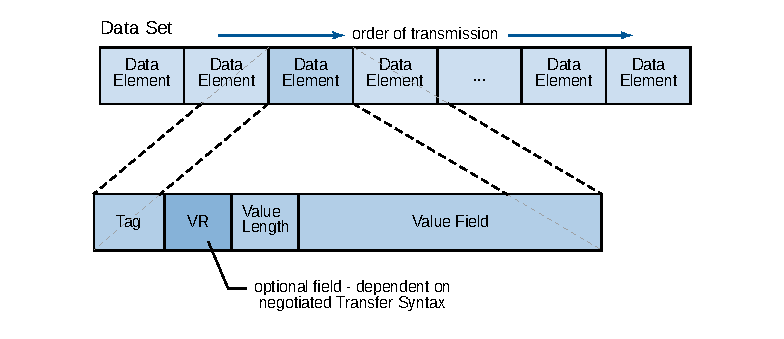
\includegraphics[trim={1.2cm 1cm 1.2cm 0.2cm},clip,width=0.7\textwidth]{img/dicom-dataelement002.pdf}
        \end{figure}

    \end{columns}
\end{frame}

\begin{frame}
    \frametitle{Cel pracy i założenia}

    \begin{alertblock}{}
        Celem pracy było zrobienie wielopratformowej przeglądarki obrazów DICOM w C++.
    \end{alertblock}

    \begin{block}{Wieloplatformowość}
        Można ją uzyskać na wiele sposobów: wirtualizacje kodu binarnego z pomocą maszyny wirtualnej takiej jak JVM, napisanie w języku skryptowym, których interpretacja kodu jest równoległa z wykonywaniem lub napisanie kodu źródłowego w taki sposób aby była możliwość jego kompilacji na wskazane platformy.
    \end{block}

    \begin{block}{Obsługa systemów}
        MS Windows, Mac OS, Linux
    \end{block}

    \begin{block}{Wczytywanie obrazów DICOM}
        Możliwość wczytania wielu plików w standardzie DICOM i ich przeglądania
    \end{block}

\end{frame}

\begin{frame}[t]
    \frametitle{Biblioteki i narzędzia}

    % Tekst
    \begin{columns}[t]
        \column{0.34\textwidth}
        \textbf{\LARGE Qt}
        \scriptsize
        jest zbiorem bibliotek i narzędzi programistycznych dedykowanych dla języków C++, QML i Java.
        Qt posiada bibliotekę do tworzenia interfejsu graficznego, oraz wiele innych rozwiązań ułatwiających programowanie obiektowe i zdarzeniowe.

        Posiadanych normy: IEC 62304:2015, IEC 61508:2010-3 7.4.4, ISO 9001:2015.

        Posiada systemy rodzicielstwa i sygnałów.

        \column{0.33\textwidth}
        \textbf{\LARGE GDCM}
        \scriptsize
        to biblioteka do obsługi standardu DICOM.
        Posiada możliwość wczytywania plików z dysku jak i z lokalizacji sieciowych oraz wczytywania plików DICOMDIR.
        Ma wbudowaną dekompresje obrazów i obsługi różnych kodowań tekstu.

        \column{0.33\textwidth}
        \textbf{\LARGE CMake}
        \scriptsize
        to wieloplatformowe narzędzie do automatycznego zarządzania procesem kompilacji programu.
        Jest to niezależne od kompilatora narzędzie pozwalające napisać jeden plik, z którego można wygenerować odpowiednie pliki budowania dla dowolnej platformy.

    \end{columns}

    % Obrazki

    \begin{columns}[c]

        \column{0.33\textwidth}
        \begin{figure}
            
\includegraphics[width=0.5\textwidth]{img/logo-qt.png}
        \end{figure}

        \column{0.34\textwidth}
        \begin{figure}
            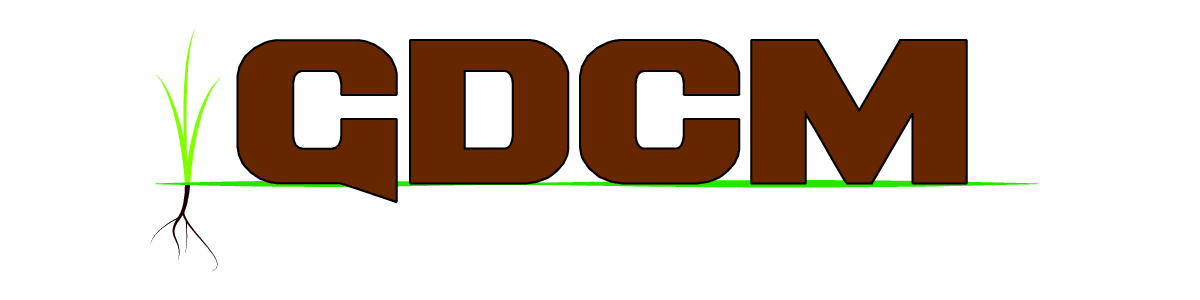
\includegraphics[width=1\textwidth]{img/logo-gdcm.png}
        \end{figure}

        \column{0.33\textwidth}
        \begin{figure}
            
\includegraphics[width=0.5\textwidth]{img/logo-cmake.png}
        \end{figure}

    \end{columns}
\end{frame}

\begin{frame}
    \frametitle{Projekt interfejsu graficznego}
    \begin{figure}
        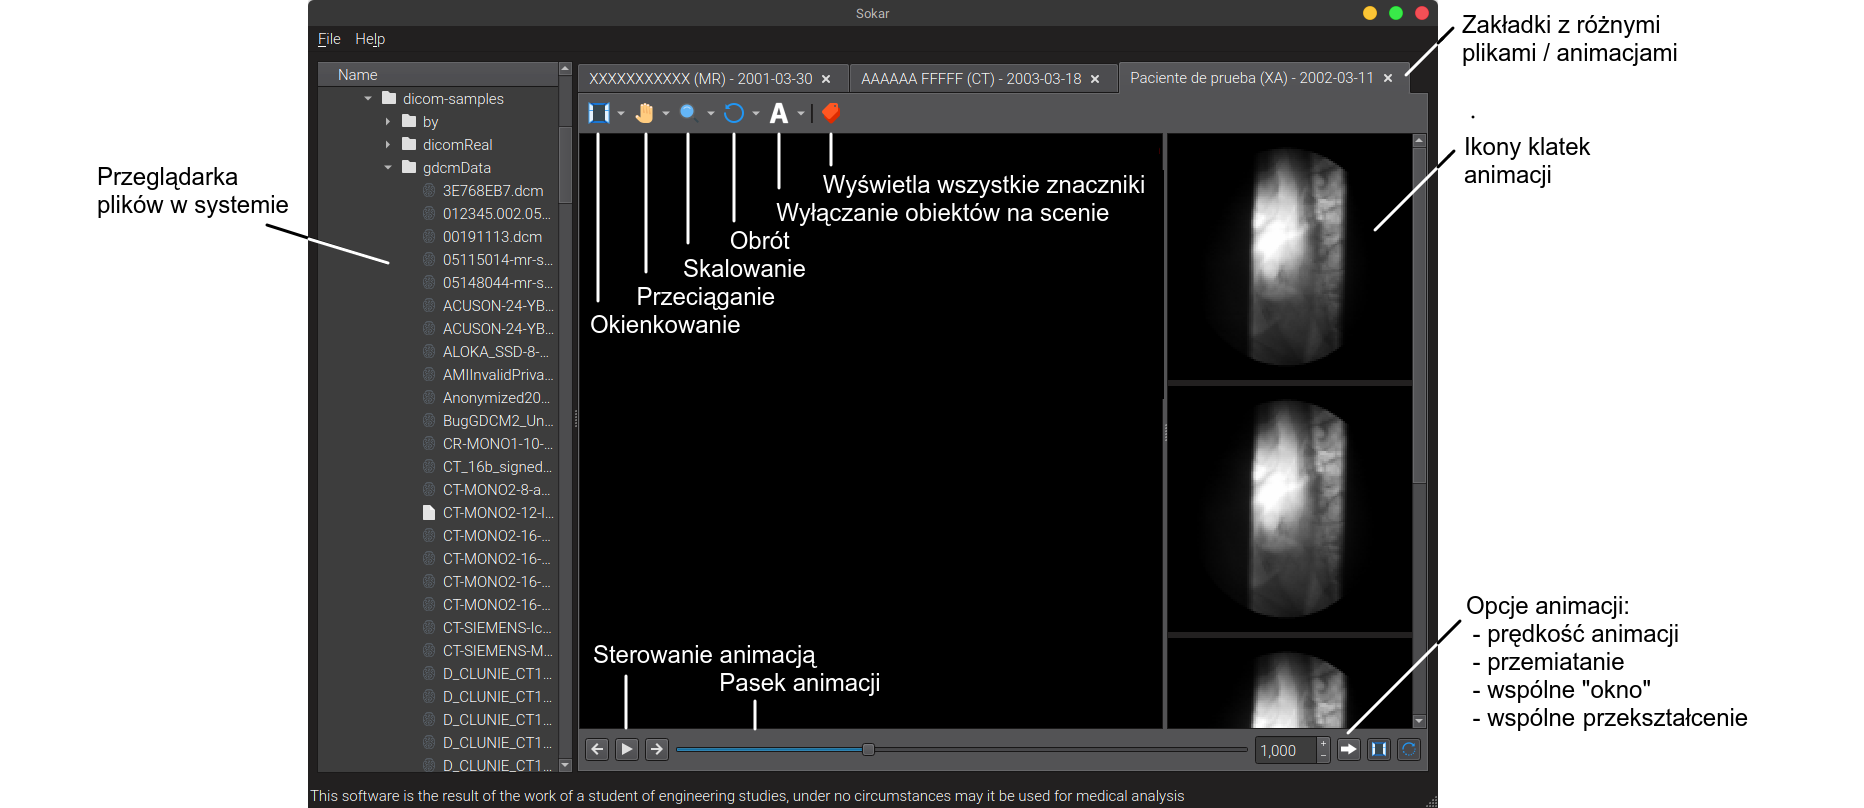
\includegraphics[height=0.8\textheight]{img/sokar-gui-004.png}
    \end{figure}
\end{frame}

\begin{frame}
    \frametitle{Projekt interfejsu graficznego}
    \setbeamertemplate{itemize items}[circle]
    \tiny
    \begin{columns}[t]

        \column{0.15\textwidth}

        Dane pacjenta:\\
        - imię i nazwisko\\
        - identyfikator\\
        - data urodzenia i wiek\\
        - opis badania\\
        - opis serii\\

        \vspace{8em}
        Litera orientacji

        \vspace{10em}
        Dane akwizycji badania\\
        różnią się w zależności od modalności


        \column{0.7\textwidth}
        \centering
        Litera orientacji
        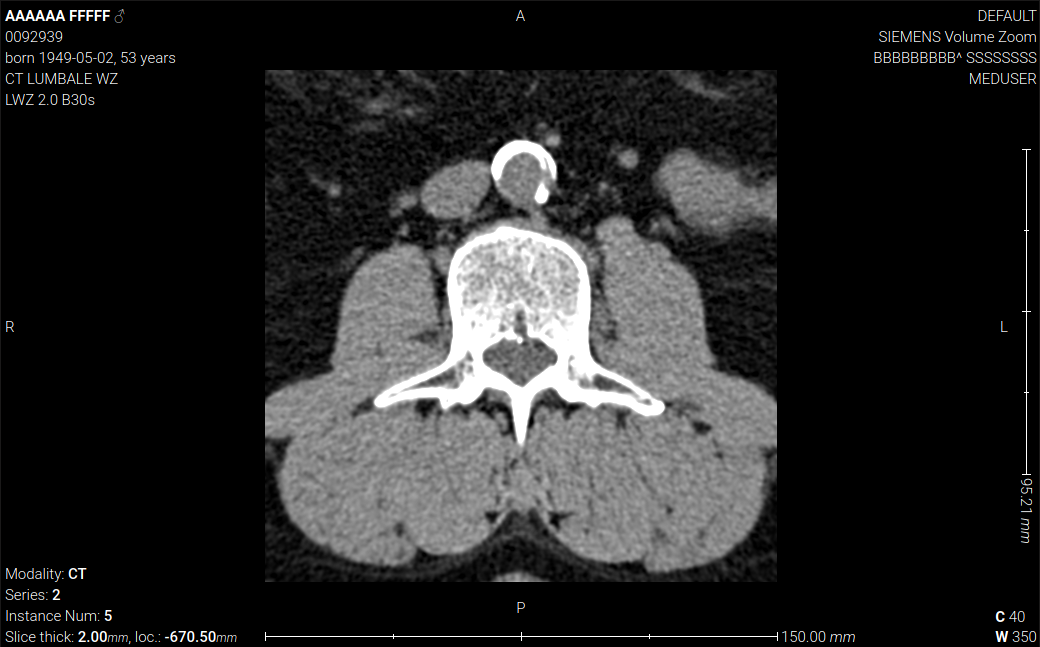
\includegraphics[width=\textwidth]{img/sokar-gui-003.png}
        Podziałka i litera orientacji

        \column{0.15\textwidth}

        Dane szpitala:\\
        - nazwa instytucji\\
        - producent i model urządzenia\\
        - lekarz wykonujący badanie\\
        - operator wykonujący badanie

        \vspace{5em}
        Litera orientacji i podziałka

        \vspace{11em}
        Parametry z jakimi jest wyświetlany obraz

    \end{columns}
\end{frame}

\begin{frame}
    \frametitle{Budowa obiektowa programu}

    \begin{columns}[c]
        \column{0.5\textwidth}

        \begin{figure}
            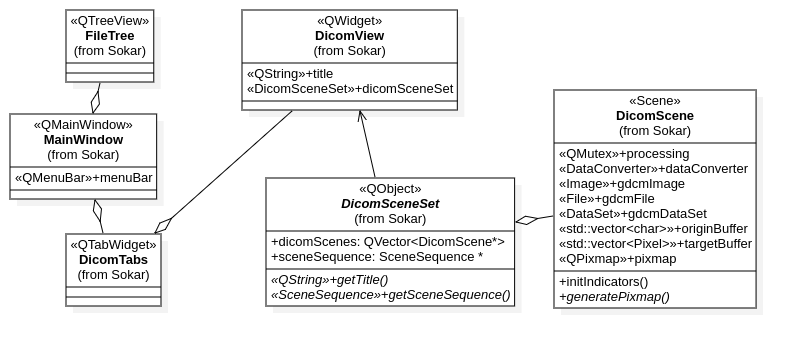
\includegraphics[width=0.95\textwidth]{img/uml/global-sturcture.png}
        \end{figure}
        \kern-2em
        \begin{figure}
            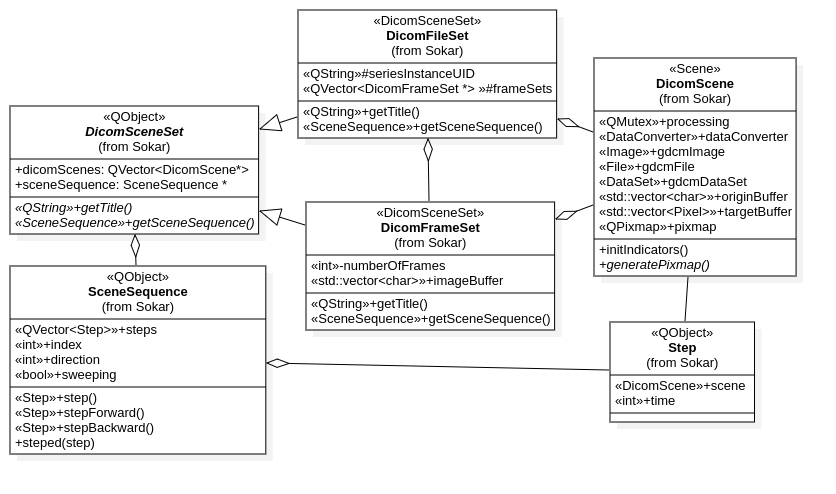
\includegraphics[width=0.95\textwidth]{img/uml/sokar-scene-sets.png}
        \end{figure}

        \column{0.5\textwidth}
        \begin{figure}
            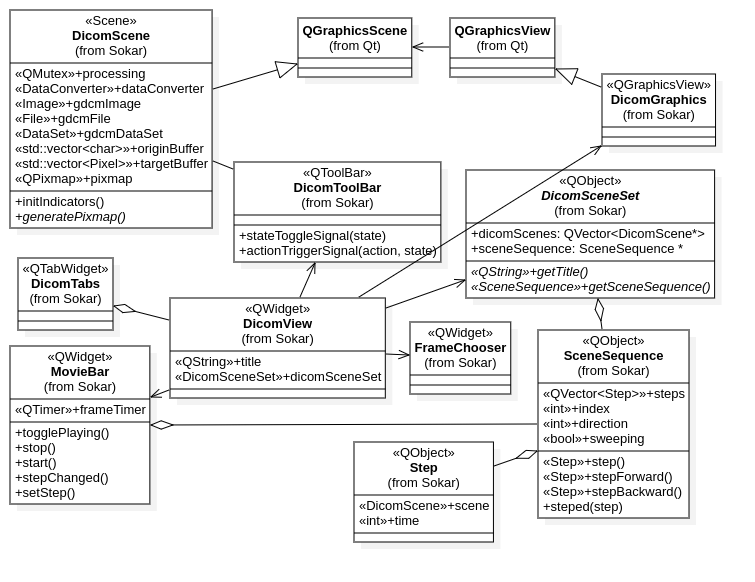
\includegraphics[width=0.95\textwidth]{img/uml/dicom-view.png}
        \end{figure}

    \end{columns}

\end{frame}

\begin{frame}[t]
    \frametitle{Dekoder DICOM}
    \begin{center}
        \footnotesize
        \def\arraystretch{1.5}
        \setlength{\tabcolsep}{5pt}
        \begin{tabular}{|l|c|c|c|c|c|c|c|c|c|c|c|c|c|c|c|c|c|c|c|c|}
            \hline
            char*  & $8b_1$                        & $8b_2$                        & $8b_3$                        & $8b_4$                        & $8b_5$                        & $8b_6$                        & $8b_7$                        & $8b_8$                        & $8b_9$ & $8b_{10}$ & $8b_{11}$ & $8b_{12}$ & $8b_{13}$ & $8b_{14}$ & $8b_{15}$ & $8b_{16}$ \\
            \hline
            int8*  & $8b_1$                        & $8b_2$                        & $8b_3$                        & $8b_4$                        & $8b_5$                        & $8b_6$                        & $8b_7$                        & $8b_8$                        & $8b_9$ & $8b_{10}$ & $8b_{11}$ & $8b_{12}$ & $8b_{13}$ & $8b_{14}$ & $8b_{15}$ & $8b_{16}$ \\
            \hline
            int16* & \multicolumn{2}{|c|}{$16b_1$} & \multicolumn{2}{|c|}{$16b_2$} & \multicolumn{2}{|c|}{$16b_3$} & \multicolumn{2}{|c|}{$16b_4$} & \multicolumn{2}{|c|}{$16b_5$} & \multicolumn{2}{|c|}{$16b_6$} & \multicolumn{2}{|c|}{$16b_7$} & \multicolumn{2}{|c|}{$16b_8$}                                                                                              \\
            \hline
            int32* & \multicolumn{4}{|c|}{$32b_1$} & \multicolumn{4}{|c|}{$32b_2$} & \multicolumn{4}{|c|}{$32b_3$} & \multicolumn{4}{|c|}{$32b_4$}                                                                                                                                                                                                                              \\
            \hline
            int64* & \multicolumn{8}{|c|}{$64b_1$} & \multicolumn{8}{|c|}{$64b_2$}                                                                                                                                                                                                                                                                                              \\
            \hline
        \end{tabular}
    \end{center}


    % \begin{lstlisting}
    % auto origin = (quint16 *) \&originBuffer[0];
    % \end{lstlisting}

\end{frame}

\begin{frame}[t]

    \frametitle{Okienkowanie}

    \vspace{-1em}

    \begin{columns}[t]
        \column{0.5\textwidth}
        \vspace{-1.0em}
        \begin{figure}
            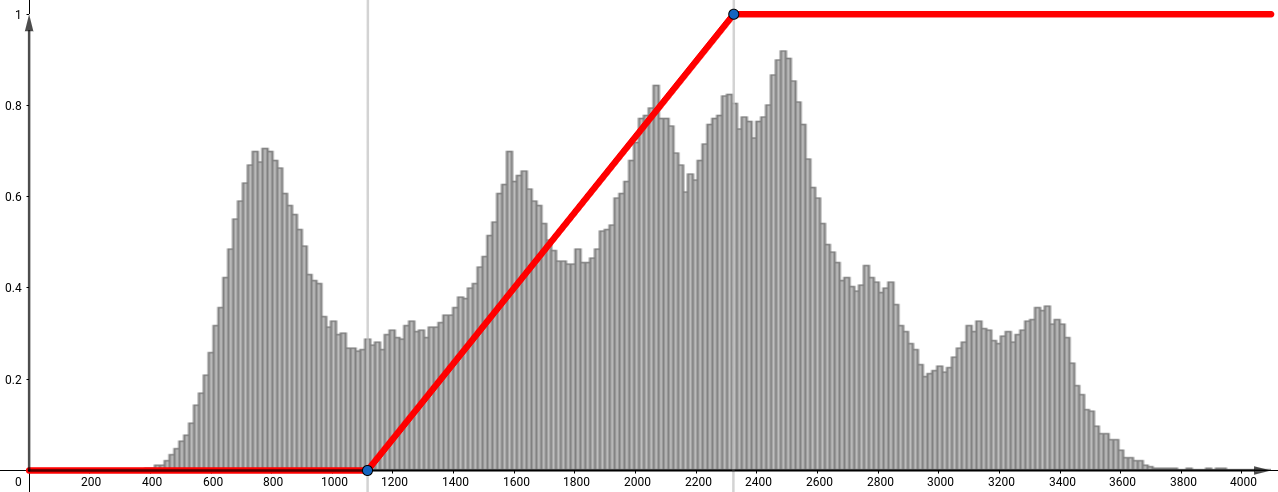
\includegraphics[width=1\textwidth]{img/windowing-chart.png}
        \end{figure}
        \vspace{-1.0em}
        \begin{figure}
            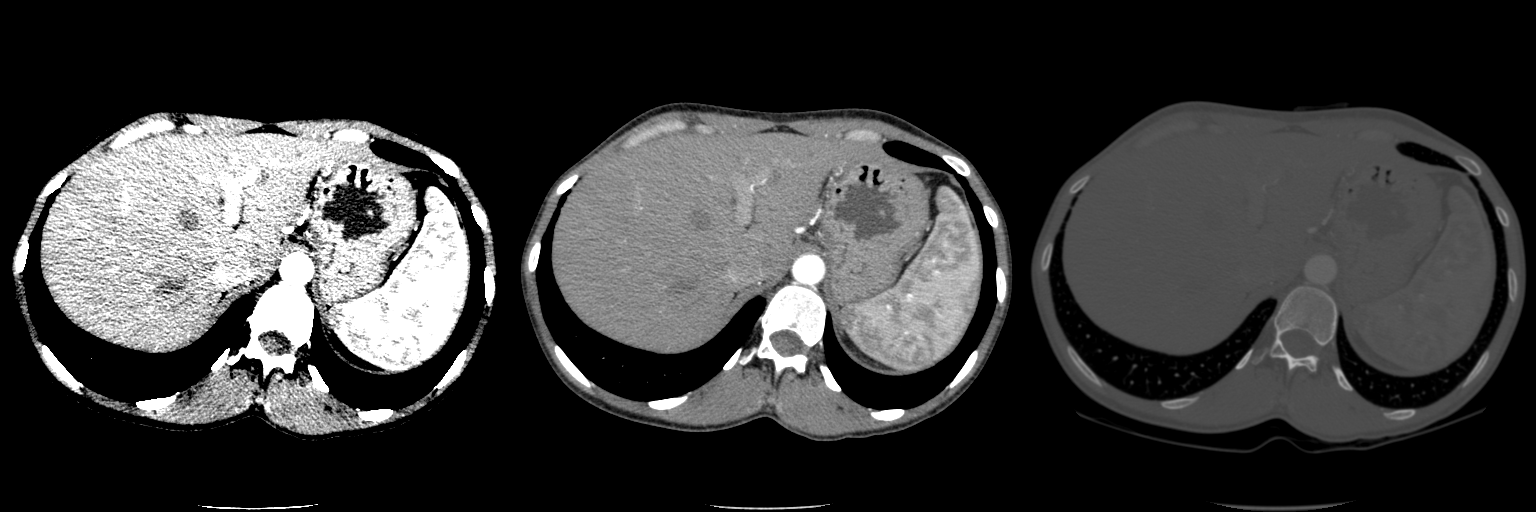
\includegraphics[trim={0 1cm 0 2cm},clip,width=1\textwidth]{img/monochrome-002.png}
        \end{figure}
        \vspace{-2.0em}
        \begin{figure}
            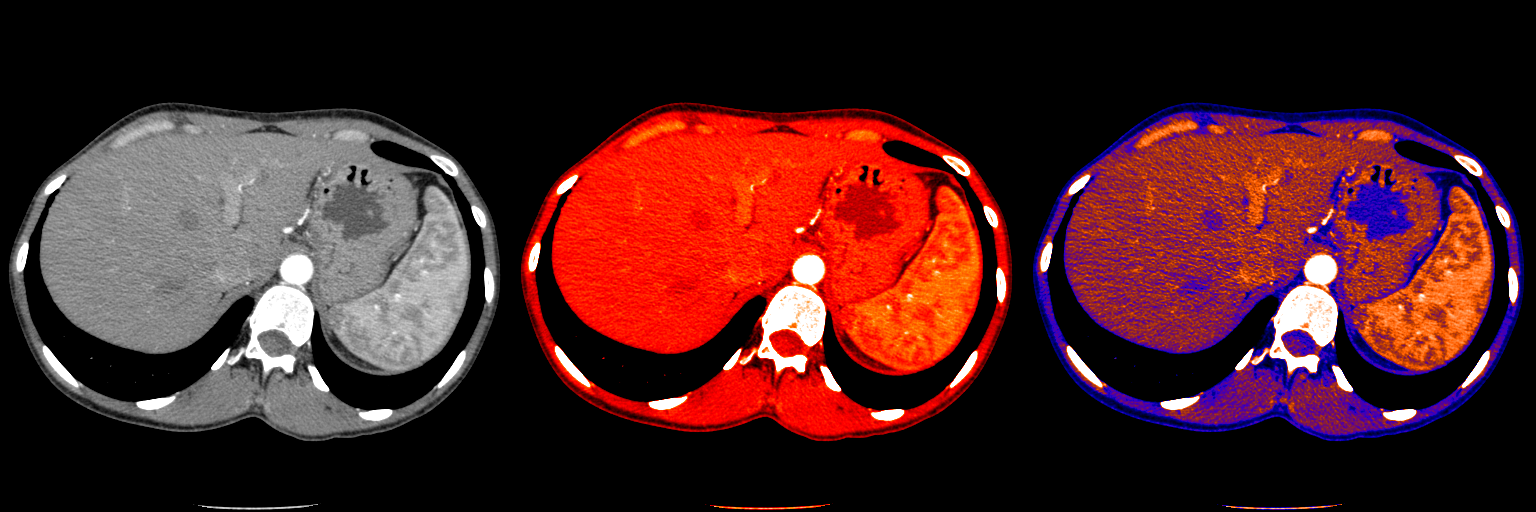
\includegraphics[trim={0 1cm 0 2cm},clip,width=1\textwidth]{img/monochrome-003.png}
        \end{figure}

        \column{0.5\textwidth}
        \tiny

        Standard \DICOM przewiduje, że wszystkie dane powinny być wyskalowane za pomocą wzoru:
        \[OutputUnits = m*SV + b\]
        \vspace{-2em}
        \begin{itemize}
            \item $m$ --- wartość z \dicomtag{RescaleSlope}{0028}{1053},
            \item $b$ --- wartość z \dicomtag{RescaleIntercept}{0028}{1052},
            \item $SV$ --- stored values --- wartość woksela z pliku,
            \item $OutputUnits$ --- wartość wynikowa.
        \end{itemize}

        \vspace{1em}
        {\normalsize Implementacja}

        \[x_0 = center - width / 2 \qquad y_0 = 1.0\]
        \vspace{-2em}
        \[x_1 = center + width / 2 \qquad y_1 = 0.0\]
        \[(OutputUnits - b ) / m = SV \]
        \[x_0 -= rescaleIntercept \qquad x_0 /= rescaleSlope\]
        \vspace{-2em}
        \[x_1 -= rescaleIntercept \qquad x_1 /= rescaleSlope\]
        \[a = (y_1 - y_0) / (x_1 - x_0) \qquad b = y_1 - a * x_1\]

        {\normalsize Tablica LUT}
        \begin{center}
            \begin{tabular}{ |c|c|c|c|c| }
                \hline
                $8 b$   & $12 b$   & $16 b$   & $32 b$    & $64 b$        \\
                \hline
                $768 B$ & $196 kB$ & $196 kB$ & $12,5 GB$ & $55*10^{6}TB$ \\
                \hline
            \end{tabular}
        \end{center}
    \end{columns}
\end{frame}

\begin{frame}[t]
    \frametitle{Orientacja pacjenta}
    \begin{columns}[t]

        \column{0.5\textwidth}
        Zapis informacji o orientacji w DICOM
        \tiny
        \[
            \begin{bmatrix}
                P_x \\ P_y \\ P_z \\ 1
            \end{bmatrix}
            =
            \begin{bmatrix}
                X_x\Delta_i & Y_x\Delta_j & 0 & S_x \\
                X_y\Delta_i & Y_y\Delta_j & 0 & S_y \\
                X_z\Delta_i & Y_z\Delta_j & 0 & S_z \\
                0           & 0           & 0 & 1
            \end{bmatrix}
            \begin{bmatrix}
                i \\ j \\ 0 \\ 1
            \end{bmatrix}
        \]
        \vspace{-1em}
        \begin{itemize}
            \item $P$ -- koordynaty woksela we współrzędnych obrazu,
            \item $S$ -- trzy wartości z elementu ze znacznikiem Image Position,
            \item $X$, $Y$ -- trzy pierwsze i trzy drugie wartości z Image Orientation,
            \item $i$ i $j$ --- oznaczają współrzędne na macierzy obrazu,
            \item $\Delta_i$ i $\Delta_j$ --- rzeczywista wielkość piksela obrazu w $mm$.
        \end{itemize}

        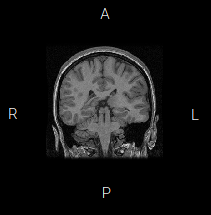
\includegraphics[height=3cm]{img/imageorientationindicator-005.png}
        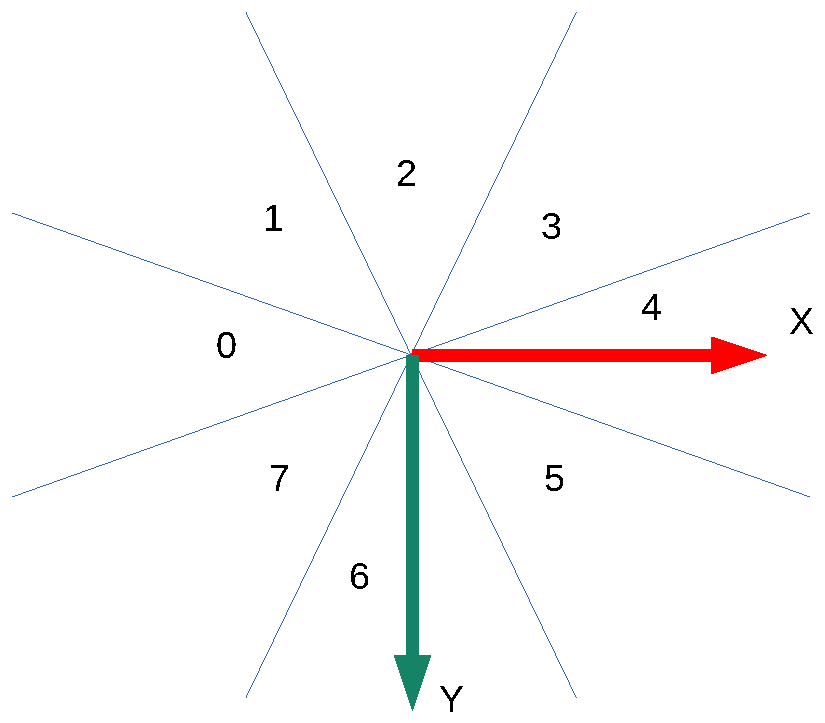
\includegraphics[height=3cm]{img/imageorientationindicator-004.pdf}

        \column{0.5\textwidth}
        Implementacja
        \tiny
        \[PatientPosition = imgMatrix * ScenePosition\]
        \vspace{-2em}
        \[imgMatrix^{-1} * PatientPosition = imgMatrix^{-1} * imgMatrix * ScenePosition\]
        \vspace{-1.5em}
        \[imgMatrix^{-1} * PatientPosition = ScenePosition\]
        \vspace{-1.5em}
        \[ScenePosition = imgMatrix^{-1} * PatientPosition\]
        \vspace{-1em}
        \begin{itemize}
            \item $imgMatrix$ --- macierz przekształcenia obrazu,
            \item $ScenePosition$ --- pozycja na obrazie, która nas interesuje,
            \item $PatientPosition$ --- jeden z punktów względem pacjenta.
        \end{itemize}
        \par
        \[
            rotateTransform*
            (
            \begin{bmatrix}
                X_x & Y_x & 0 & 0 \\
                X_y & Y_y & 0 & 0 \\
                X_z & Y_z & 0 & 0 \\
                0   & 0   & 0 & 1
            \end{bmatrix}
            * PatientPosition)
        \]
        \hspace*{-5em}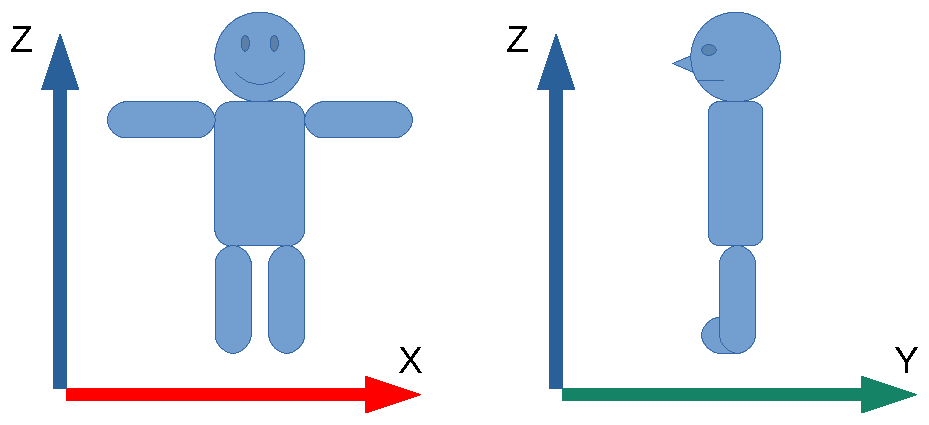
\includegraphics[height=2cm]{img/imageorientationindicator-003.pdf}
    \end{columns}


\end{frame}

\begin{frame}
    \frametitle{Funckje przeglądarki}
    \begin{itemize}
        \item Podstawowe operacje na orazie
        \item Okienkowanie i pseudokolorowanie
        \item Możliwość wczytania wielu plików i animacji
    \end{itemize}
\end{frame}

\begin{frame}
    \frametitle{Wnioski}
    przetestowano

    automatycznie sie kompiluje

    intefjes jest podobny

\end{frame}

\end{document}
